\documentclass{article}
\usepackage[margin=0.25cm,papersize={19cm,9.8cm}]{geometry}
\usepackage{amsmath,amssymb}
\usepackage{tikz}
\usetikzlibrary{arrows.meta,positioning}
\pagestyle{empty}

\definecolor{rank0Col}{RGB}{24, 100, 171}    % Deep Blue
\definecolor{rank1Col}{RGB}{43, 138, 62}     % Forest Green
\definecolor{rank2Col}{RGB}{217, 119, 6}     % Warm Amber
\definecolor{rank3Col}{RGB}{128, 43, 179}    % Royal Purple
\definecolor{arrowCol}{RGB}{224, 49, 49}     % Crimson Red
\definecolor{axisCol}{RGB}{120, 120, 120}    % Axis gray

\begin{document}
\centering
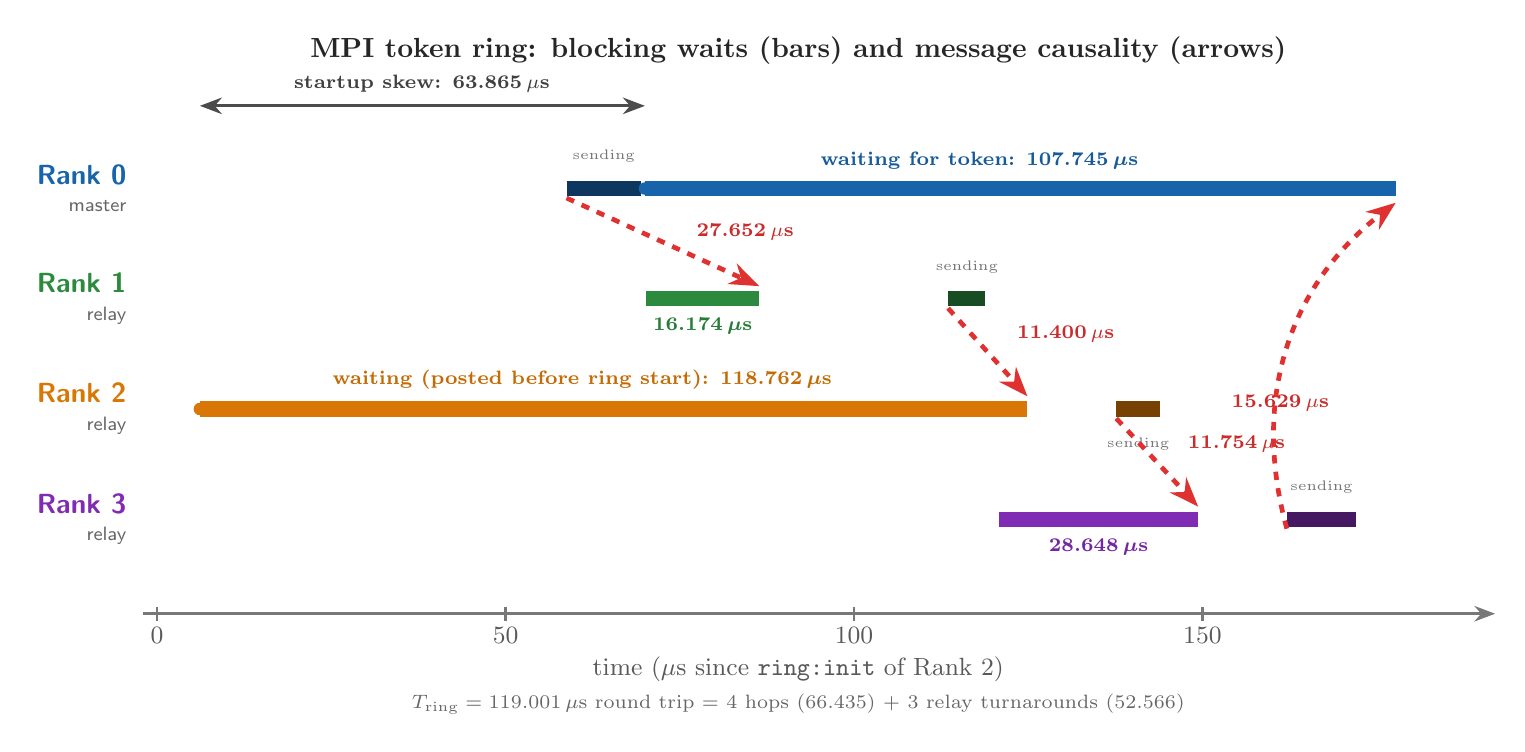
\begin{tikzpicture}[
    font=\sffamily,
    >=Stealth,
    x=0.0885cm,
    waitBar/.style={line width=5.5pt},
    sendBar/.style={line width=5.5pt, color=black!55},
    hopArrow/.style={->, line width=1.7pt, draw=arrowCol, dashed}
]

    % ---------------- time axis ----------------
    \draw[->, line width=1pt, draw=axisCol] (-2,0) -- (192,0);
    \foreach \x/\lab in {0/{0}, 50/{50}, 100/{100}, 150/{150}} {
        \draw[line width=0.8pt, draw=axisCol] (\x, -0.09) -- (\x, 0.09);
        \node[below=1.5pt, font=\small, text=black!65] at (\x, 0) {\lab};
    }
    \node[below=12pt, font=\small, text=black!65] at (92, 0)
        {time ($\mu$s since \texttt{ring:init} of Rank 2)};

    % ---------------- row positions ----------------
    \def\yZero{5.4}
    \def\yOne{4.0}
    \def\yTwo{2.6}
    \def\yThree{1.2}

    % Rank labels (left margin)
    \node[left, align=right, text=rank0Col] at (-3, \yZero)
        {\textbf{Rank 0}\\[-2pt]{\scriptsize\textcolor{black!60}{master}}};
    \node[left, align=right, text=rank1Col] at (-3, \yOne)
        {\textbf{Rank 1}\\[-2pt]{\scriptsize\textcolor{black!60}{relay}}};
    \node[left, align=right, text=rank2Col] at (-3, \yTwo)
        {\textbf{Rank 2}\\[-2pt]{\scriptsize\textcolor{black!60}{relay}}};
    \node[left, align=right, text=rank3Col] at (-3, \yThree)
        {\textbf{Rank 3}\\[-2pt]{\scriptsize\textcolor{black!60}{relay}}};

    % ---------------- Rank 0 (blue) ----------------
    \draw[sendBar, draw=rank0Col!55!black] (58.744, \yZero) -- (69.423, \yZero);
    \draw[waitBar, draw=rank0Col] (70.000, \yZero) -- (177.745, \yZero);
    \node[above=3.5pt, font=\scriptsize, text=rank0Col!90!black] at (118, \yZero)
        {\textbf{waiting for token: 107.745\,$\boldsymbol{\mu}$s}};
    \node[above=1pt, font=\tiny, text=black!55] at (64.1, \yZero+0.17) {sending};

    % ---------------- Rank 1 (green) ----------------
    \draw[waitBar, draw=rank1Col] (70.222, \yOne) -- (86.396, \yOne);
    \draw[sendBar, draw=rank1Col!55!black] (113.497, \yOne) -- (118.863, \yOne);
    \node[below=3.5pt, font=\scriptsize, text=rank1Col!90!black] at (78.3, \yOne)
        {\textbf{16.174\,$\boldsymbol{\mu}$s}};
    \node[above=1pt, font=\tiny, text=black!55] at (116.2, \yOne+0.17) {sending};

    % ---------------- Rank 2 (amber) ----------------
    \draw[waitBar, draw=rank2Col] (6.135, \yTwo) -- (124.897, \yTwo);
    \draw[sendBar, draw=rank2Col!55!black] (137.640, \yTwo) -- (143.973, \yTwo);
    \node[above=3.5pt, font=\scriptsize, text=rank2Col!90!black] at (61, \yTwo)
        {\textbf{waiting (posted before ring start): 118.762\,$\boldsymbol{\mu}$s}};
    \node[below=2pt, font=\tiny, text=black!55] at (140.8, \yTwo-0.17) {sending};

    % ---------------- Rank 3 (purple) ----------------
    \draw[waitBar, draw=rank3Col] (120.746, \yThree) -- (149.394, \yThree);
    \draw[sendBar, draw=rank3Col!55!black] (162.116, \yThree) -- (172.087, \yThree);
    \node[below=3.5pt, font=\scriptsize, text=rank3Col!90!black] at (135.1, \yThree)
        {\textbf{28.648\,$\boldsymbol{\mu}$s}};
    \node[above=1pt, font=\tiny, text=black!55] at (167.1, \yThree+0.17) {sending};

    % ---------------- hop arrows (send_entry -> recv_exit) ----------------
    \draw[hopArrow] (58.744, \yZero-0.12) -- (86.396, \yOne+0.16);
    \node[right, font=\scriptsize\bfseries, text=arrowCol!90!black, align=left]
        at (76, 4.85) {27.652\,$\mu$s};

    \draw[hopArrow] (113.497, \yOne-0.12) -- (124.897, \yTwo+0.16);
    \node[right, font=\scriptsize\bfseries, text=arrowCol!90!black, align=left]
        at (122, 3.55) {11.400\,$\mu$s};

    \draw[hopArrow] (137.640, \yTwo-0.12) -- (149.394, \yThree+0.16);
    \node[right, font=\scriptsize\bfseries, text=arrowCol!90!black, align=left]
        at (146.5, 2.15) {11.754\,$\mu$s};

    \draw[hopArrow] (162.116, \yThree-0.12) to[bend left=34]
        node[pos=0.42, below=3pt, font=\scriptsize\bfseries, text=arrowCol!90!black]
        {15.629\,$\mu$s} (177.745, \yZero-0.18);

    % ---------------- startup skew bracket ----------------
    \draw[<->, line width=1.1pt, draw=black!70]
        (6.135, 6.45) -- (70.000, 6.45);
    \node[above=1.5pt, font=\scriptsize\bfseries, text=black!75] at (38, 6.45)
        {startup skew: 63.865\,$\mu$s};

    \node[circle, fill=rank2Col, inner sep=1.6pt] at (6.135, \yTwo) {};
    \node[circle, fill=rank0Col, inner sep=1.6pt] at (70.000, \yZero) {};

    % ---------------- title ----------------
    \node[font=\normalsize\bfseries, text=black!85] at (92, 7.15)
        {MPI token ring: blocking waits (bars) and message causality (arrows)};
    \node[font=\scriptsize, text=black!60] at (92, -1.15)
        {$T_{\text{ring}} = 119.001\,\mu\text{s}$ round trip $=$ 4 hops $(66.435)$ $+$ 3 relay turnarounds $(52.566)$};

\end{tikzpicture}
\end{document}
